% !Mode:: "TeX:UTF-8"
% !Mode:: "TeX:UTF-8"
\newcommand{\thepage}{} % to silence a hyperref warning about pdfpagelabels
\RequirePackage[]{silence}
\WarningsOff[hyperref]
\PassOptionsToPackage{log-declarations=false}{xparse}
%\RequirePackage[l2tabu, orthodox]{nag}
\RequirePackage{luatex85} % to make \pdf...= commands work with LuaTeX
\documentclass[aspectratio=169,t]{beamer}
\usepackage{ifthen}
\usepackage[T1]{fontenc}
\usepackage{iftex}
\ifLuaTeX
 \usepackage{fontspec}
 \setmainfont[Ligatures=TeX]{Source Sans Pro}
\else
 \usepackage[utf8]{inputenc}
\fi
\usepackage{german}
\usepackage{newunicodechar}
\newunicodechar{€}{\texteuro}
\newunicodechar{ß}{\ss}
\renewcommand{\SS}{\iffontchar\font"1E9E \symbol{"1E9E}\else SS\fi}
\usepackage{ellipsis}
\usepackage{microtype}
\usepackage{listings}
\usepackage{sourcecodepro}
\lstset{language=Python, basicstyle=\ttfamily}
\usepackage{amsfonts}
\usepackage{amssymb}
\usepackage{amsthm}
\usepackage{fancyhdr}
\usepackage{graphicx}

\newtheorem{proposition}[theorem]{Proposition}

\DeclareMathOperator*{\argmax}{argmax}
\DeclareMathOperator{\supp}{supp}
\newcommand{\E}{\ensuremath{\mathbb{E}}}
\newcommand{\V}{\ensuremath{\mathbb{V}}}

\setbeamercolor{emph}{fg=purple}
\renewcommand<>{\emph}[1]{%
  {\usebeamercolor[fg]{emph}\only#2{\itshape}#1}%
}



\hypersetup{draft=false,colorlinks=false,pdfpagemode=UseOutlines,plainpages=false,
            breaklinks=true,bookmarksnumbered=true,pdfborder=0 0 0,
            pdftitle={Data Science SoSe 2026 HHU},
            pdfauthor={Konrad Voelkel},
            pdfsubject={data science}}

%\documentclass[aspectratio=169,t]{beamer}
\usetheme{hhubeamer} % put the hhu-beamer-theme in /usr/share/texmf/tex/latex/beamer/themes/

% -------------------- Code listings config --------------------
% Define custom colors for syntax highlighting
\definecolor{codegreen}{rgb}{0,0.6,0}
\definecolor{codegray}{rgb}{0.5,0.5,0.5}
\definecolor{codepurple}{rgb}{0.58,0,0.82}
\definecolor{backcolour}{rgb}{0.96,0.96,0.94} % Very light gray/beige
% Configure the listings package
\lstset{
    language=Python,
    backgroundcolor=\color{backcolour},   
    commentstyle=\color{codegreen}\itshape,
    keywordstyle=\color{blue}\bfseries,
    numberstyle=\tiny\color{codegray},
    stringstyle=\color{codepurple},
    basicstyle=\ttfamily\footnotesize, % Use a monospaced font
    breakatwhitespace=false,         
    breaklines=true,      
             % Enable automatic line breaking
    captionpos=b,                      % Caption at the bottom
    keepspaces=true,                 
    numbers=left,                      % Line numbers on the left
    numbersep=10pt,                    % Distance of line numbers from the code
    showspaces=false,                
    showstringspaces=false,            % Don't show weird underscores in strings
    showtabs=false,                  
    tabsize=4,
    frame=single,                      % Add a subtle border around the code
    rulecolor=\color{black!20},        % Border color
  }

\event[]{}
\author[Sommersemester 2026]{Dr. Konrad Völkel, Sommersemester 2026}

%\title{Data Science, VL 1}
%\date{16.04.2026}


%%% Local Variables:
%%% mode: latex
%%% TeX-master: t
%%% End:


\title{Data Science, VL 2}
\date{21.04.2026}

\begin{document}

\begin{frame}
  \titlepage
\end{frame}

\section{Recap}

\begin{frame}\frametitle{Erinnerung: Wahrscheinlichkeitsmaß}
  Sei $(\Omega, \mathcal{F})$ ein Ereignisraum, also $\mathcal{F}$ eine Menge von Ereignissen\\
  (sodass die Regeln ``WAHR'',``NICHT'',``ODER'' für Ereignisse gelten).

  Dann heißt eine Abbildung
  \[P \colon \mathcal{F} \to [0,1]\]
  \emph{Wahrscheinlichkeitsmaß}, wenn
  \begin{itemize}
    \item $P(\Omega) = 1$ (Normierung) und
    \item für paarweise disjunkte Ereignisse $A_i \in \mathcal{F}$ gilt
      \emph{$\sigma$-Additivität}:
      \[P\left( \bigcup_{i} A_i\right) = \sum_i P\left(A_i\right).\]
  \end{itemize}
\end{frame}

\begin{frame}\frametitle{Beweis an der Tafel}
  Wir beweisen an der Tafel aus den Axiomen für Wahrscheinlichkeitsmaße (Normierung, $\sigma$-Additivität):
  \begin{enumerate}
    \item $P(\emptyset) = 0$
    \item $P(A\cup B) =P(A) + P(B) - P(A\cap B)$
    \item $A \subset B \Rightarrow P(A) \leq P(B)$
  \end{enumerate}
\end{frame}

\begin{frame}\frametitle{Beispiel an der Tafel}
  Wir rechnen mit dem Ergebnis eines Zufallsexperiments $X$ (z.B. $2\cdot X$)
\end{frame}

\section{Zufallsvariable - Definition}

\begin{frame}\frametitle{Definition Zufallsvariable}
  Eine Abbildung $X \colon \Omega' \to \Omega$ zwischen zwei Ereignisräumen $(\Omega',\mathcal{F}')$ und $(\Omega,\mathcal{F})$ heißt \emph{Zufallsvariable}, wenn für jedes Ereignis $A \in \mathcal{F}$ auch das sogenannte \emph{Urbild} $X^{-1}(A) \subseteq \Omega'$ ein Ereignis ist, also
  \[X^{-1}(A) = \{ \omega' \in \Omega' \ : \ X(\omega') \in A \} \in \mathcal{F}'.\]
\end{frame}


\section{Zufall und Zufallsvariable}

\subsection{Zufallsquelle}

\begin{frame}
  \frametitle{Wo kommt der Zufall her?}
  \framesubtitle{Oder: wo kommt der Zufall hin?}
  \begin{itemize}[<+->]
    \item A priori gibt es keinen Zufall!
    \item Wahrscheinlichkeiten als Häufigkeiten in beobachteten Daten: Zufall als Modell.
    \item Daten erfassen in der Welt: deterministisch.
    \item Sampling / Stichproben ziehen aus Daten: simulierter Zufall.
    \item Sampling aus Wahrscheinlichkeitsmodellen: simulierter Zufall.
    \end{itemize}
    \uncover<3->{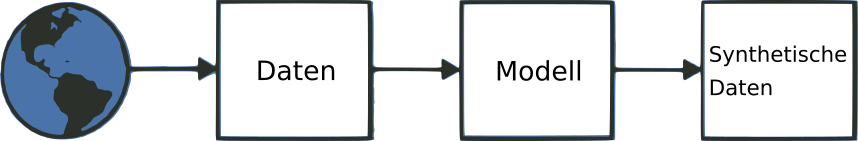
\includegraphics[width=12cm]{figures/dsprozess-simplified-2.png}}
\end{frame}

\begin{frame}
  \frametitle{Beispiel Würfelwurf}
  \framesubtitle{Wo kommen die Daten her?}
  \begin{itemize}[<+->]
  \item Weltausschnitt: Wir wählen einen konkreten Würfel aus allen Dingen aus.
  \item Rohdaten: Wir zeichnen die 3D-Koordinaten der Würfelecken (relativ zu einem festen Bezugspunkt) auf - für jeden Moment in der Welt 8 Eckpunkte, also 8*3 reelle Zahlen.
  \item Daten: Wenn bei der Erfassung etwas schief ging (Messfehler, Übertragungsfehler), bereinigen wir die Daten.
    \end{itemize}
    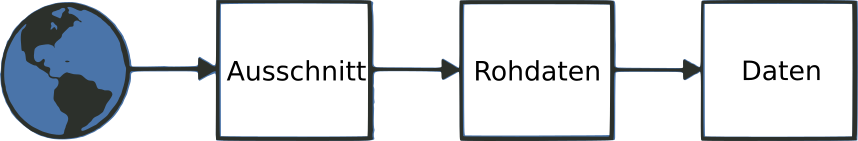
\includegraphics[width=12cm]{figures/dsprozess-simplified-1.png}
\end{frame}

\begin{frame}
  \frametitle{Beispiel Würfelwurf}
  \framesubtitle{Was machen wir mit den Daten?}
  \begin{itemize}[<+->]
  \item Daten: das, was wir an scheinbar korrekten Daten in unserem Weltausschnitt gemessen haben (8*3 reelle Zahlen).
  \item Transformierte Daten: Aus den 3D-Koordinaten der Würfelecken berechnen wir 3D-Koordinaten des Mittelpunkts und die Rotationswinkel relativ zu einem Idealzustand (z.B. 6 oben, 2 vorne), also 3+3 reelle Zahlen.
  \item  Zielgröße: welche Augenzahl zeigt der Würfel?
    \end{itemize}
    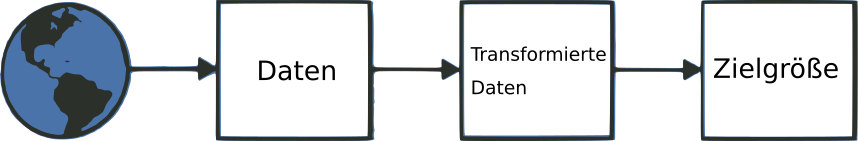
\includegraphics[width=12cm]{figures/dsprozess-simplified-3.png}
\end{frame}

\begin{frame}
  \frametitle{Beispiel Würfelwurf}
  \framesubtitle{Wo sind die Zufallsvariablen, wo der Zufall?}
  \begin{itemize}[<+->]
  \item Wir können die Welt als zufällig oder deterministisch ansehen. Eigentlich egal, denn wir wissen nicht alles über die Welt. Vom Unbekannten wissen wir nur so grob die Verteilung (Zufall als Modellierungswerkzeug).
  \item Von der Welt zu den Daten, das ist eine Abbildung. Das ist eine Zufallsvariable!
    \item Von den Daten zu den transformierten Daten, weiter zur Zielgröße, das sind ebenfalls Abbildungen. Auch Welt $\to$ Zielgröße (die Verkettung der Abbildungen) ist eine Zufallsvariable.
    \end{itemize}
    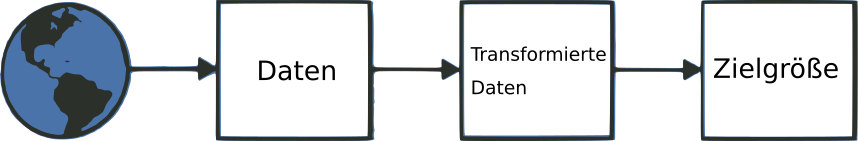
\includegraphics[width=12cm]{figures/dsprozess-simplified-3.png}
  \end{frame}

  \begin{frame}
  \frametitle{Beispiel Würfelwurf}
  \framesubtitle{Die Zielgröße ``Augenzahl'' als Zufallsvariable}
  \Huge{   \[ X \colon  \text{Welt} = \Omega' \longrightarrow \Omega = \{1,2,3,4,5,6\}\] }
  \normalsize
  Bei einem fairen Würfel ist
  \[P(X = 6) = P_{\text{Welt}}\left( w \in \Omega' : X(w) = 6\right) = \dfrac{1}{6}, \]
  denn es gibt genau so viele Weltzustände $w$ die einer $6$ entsprechen, wie jeweils solche die einer $1$, $2$, $3$, $4$ oder $5$ entsprechen.
\end{frame}


\subsection{Formalismus}

\begin{frame}
  \frametitle{Messbare Abbildung}
  Wenn $\mathcal{Y}$ und $\mathcal{X}$ Mengen sind, die eine $\sigma$-Algebra tragen (d.h. vor Allem, dass manche Teilmengen $A \subset \mathcal{X}$ bzw. $B \subset \mathcal{Y}$ als messbare Mengen [oder auch Ereignisse] bezeichnet werden), dann heisst eine Abbildung
  \[f \colon \mathcal{Y} \to \mathcal{X}\]
  \alert{messbar}, wenn zu jeder messbaren Menge $A \subset \mathcal{X}$ auch das Urbild
  \[f^{-1}(A) := \{ y \in Y : f(y) \in A \} \subseteq \mathcal{Y}\]
  eine messbare Menge in $\mathcal{Y}$ ist.
\end{frame}

\begin{frame}
  \frametitle{Induziertes Maß (Bildmaß)}
  Wenn auf dem Definitionsbereich von $f \colon \mathcal{Y} \to \mathcal{X}$ ein Maß $P_{\mathcal{Y}}$ definiert ist,
  dann lässt sich auch auf dem Wertebereich ein (neues!) Maß $P_{\mathcal{X}} := P_f$ definieren:
    
    Für $A \subset \mathcal{X}$ setze
    \[P_f(A) := P_{\mathcal{Y}}\left( f^{-1}(A) \right) = P_{\mathcal{Y}}\left( y \in Y : f(y) \in A \right). \]
    Das ist das \alert{Bildmaß} oder auch einfach \alert{die Verteilung von f}.
\end{frame}

\begin{frame}
  \frametitle{Zufallsvariable}
  Wenn $\mathcal{Y}$ ein Wahrscheinlichkeitsraum ist, d.h. es ist ein Wahrscheinlichkeitsmaß $P$ definiert,
  und eine Menge $\mathcal{X}$ trägt eine $\sigma$-Algebra (z.B. die Potenzmenge),
  dann nennt man jede messbare Abbildung $f \colon \mathcal{Y} \to \mathcal{X}$ eine \alert{Zufallsvariable} und $P_f$ die \alert{Verteilung der Zufallsvariablen}.
\end{frame}

\begin{frame}
  \frametitle{Beispiel gerade Würfelaugen}
  \uncover<+->{
  Eine weitere (messbare) Abbildung:
  \[g \colon \Omega = \{1,2,3,4,5,6\} \to G = \{\text{gerade}, \text{ungerade}\} \simeq \{0, 1\}\]
  \[1,3,5 \mapsto \text{ungerade} = 1,\]
  \[2,4,6 \mapsto \text{gerade} = 0.\]
  }
    \uncover<+->{
      Dann ist $P_g(\{\text{gerade}\}) = P_\Omega\left( g^{-1}(\{ \text{gerade} \}) \right) = P_\Omega(\{2,4,6\}) = \dfrac{1}{2}$.
      }
  
  \uncover<+->{
    Wenn $X : \text{Welt} \to \Omega$ die ursprüngliche Zufallsvariable ist, dann ist auch $g(X)$ eine Zufallsvariable:
    \[g(X) = g \circ X \colon \text{Welt} \to G = \{\text{gerade}, \text{ungerade}\} \]
  }
  \uncover<+->{
    Dabei ist $P_{g(X)} = P_g$. Es kommt also nicht so sehr auf den Definitionsbereich an.
  }
\end{frame}

\begin{frame}
  \frametitle{Beispiel Würfelaugen größergleich fünf}
\uncover<+->{
  Eine weitere Abbildung:
  \[f \colon \Omega = \{1,2,3,4,5,6\} \to B = \{\text{ja}, \text{nein}\}\]
  \[1,2,3,4 \mapsto \text{nein},\]
  \[5,6 \mapsto \text{ja}.\]
}
  \uncover<+->{
    Da die Urbilder von nein und ja jeweils messbare Mengen sind ($\Omega$ endlich $\Rightarrow$ kann alle Mengen messbar nennen): $f$ ist eine Zufallsvariable.
  }
    \uncover<+->{
      \[P_f\left(\{\text{nein}\}\right) = P_\Omega\left(\{1,2,3,4\}\right) = P_\Omega\left(\{1\} \cup \{2\} \cup \{3\} \cup \{4\}\right) = \sum_{i=1}^4 P_\Omega\left(\{i\}\right) = \dfrac{4}{6} = \dfrac{2}{3}.\]
      }
\end{frame}



\section{Diskrete Verteilungen als Modelle}

\begin{frame}
  \frametitle{pmf}
\uncover<+->{
  Für endliche (oder abzählbar unendliche) Mengen $A \subseteq \Omega$ haben wir schon festgestellt:
  \[P(A) = P\left( \bigcup_{a \in A} \{a\}  \right) = \sum_{a \in A} P\left(\{a\}\right) \uncover<3->{ = \sum_{a \in A} p(a) }\]
}
\uncover<+->{
  Die Abbildung $p \colon \Omega \to [0,1]$ mit Definition
  \[p(x) := P\left(\{x\}\right)\]
  kodiert also bereits $P$ für alle abzählbar unendlichen oder kleineren Teilmengen.
}
\uncover<+->{
  Wenn $\Omega$ selbst höchstens abzählbar unendlich ist, lässt sich $P$ aus $p$ vollständig berechnen.
  Die Funktion $p$ heißt \alert{probability mass function} (pmf, Wahrscheinlichkeitsmassefunktion).
  }
\end{frame}

\begin{frame}
  \frametitle{Beispiel pmf}
\uncover<+->{
  Sei $\Omega$ eine Menge (potentiell unendlich) und $\omega \in \Omega$ ein Element.
  Dann ist $P \colon \mathcal{P}(\Omega) \to [0,1]$ mit
  \[P(A) := \begin{cases} 1 & \omega \in A \\ 0 & \omega \notin A \end{cases} \]
  eine Wahrscheinlichkeitsverteilung (ein W-Maß) definiert,
  die \alert{Dirac-Verteilung mit Masse an $\omega$}.
}
\uncover<+->{
  Die Abbildung $p \colon \Omega \to [0,1]$ mit Definition
  \[p(x) := \begin{cases} 1 & x=\omega \\ 0 & x \neq \omega \end{cases}\]
  ist eine pmf für $P$, wenn $\Omega$ höchstens abzählbar unendlich ist.
}
\end{frame}

\begin{frame}
  \frametitle{Induzierte pmf}
\uncover<+->{
  Seien $\Omega, \Omega'$ höchstens abzählbar unendliche Mengen und $P$ ein W-Maß auf $\Omega'$ mit pmf $p$.
  Zu einer messbaren Abbildung
  \[f \colon \Omega' \to \Omega\]
}
\uncover<+->{
  ist die Abbildung $p_f \colon \Omega \to [0,1]$ mit
  \[p_f(\omega) := \sum_{x \in \Omega' : f(x)=\omega} p(x)\]
  eine pmf für die durch $f$ von $P$ induzierte Verteilung $P_f$ auf $\Omega$.
}
\end{frame}

\begin{frame}
  \frametitle{Wahrscheinlichkeitsvektor}
\uncover<+->{
  Wenn $\Omega$ eine angeordnete endliche Menge $\Omega = \{\omega_1,\dots,\omega_n\}$ ist,
  lässt sich eine pmf $p$ über den Vektor $(p_i)$ der $p_i := p(\omega_i)$ kodieren.
}

\uncover<+->{
  Es ist dann $\sum_{i=1}^n p_i = 1$. Jeder solche Vektor mit $0 \leq p_i \leq 1$ definiert eine pmf auf $\Omega$ und wird
  \alert{Wahrscheinlichkeitsvektor} genannt.
}
\end{frame}

\begin{frame}
  \frametitle{Beispiel Bernoulli-Verteilung}
\begin{itemize}[<+->]
\item  Wenn $\Omega = \{\omega_1,\omega_2\}$,
  wählen wir oft $\Omega = \{0,1\}$ und für jeden Wahrscheinlichkeitsvektor $p = (p_0,p_1)$ gilt $p_0 = 1-p_1$,
  weshalb wir oft nur $p=p_1$ notieren.
\item  Die Verteilung auf $\{0,1\}$, die durch ein $p \in [0,1]$ mit $p = P(\{1\})$ definiert ist,
  heißt \alert{Bernoulli-Verteilung} zum Parameter $p$.
\item  Für $p=0.5$ ist das eine Gleichverteilung, für $p=0$ und $p=1$ jeweils Dirac-Verteilungen.
  Alles andere modelliert unfaire Münzwürfe.
\end{itemize}
\end{frame}

\begin{frame}
  \frametitle{Menge aller Wahrscheinlichkeitsvektoren}
\uncover<+->{
  Die Menge
  \[\Delta_n := \left\{ p \in \mathbb{R}^n : 0 \leq p_i \leq 1,\ \sum_{i=1}^n p_i = 1 \right\}\]
  parametrisiert alle Verteilungen auf einer $n$-elementigen angeordneten Menge.
}

\uncover<+->{
  Für $n=2$ ist $\Delta_2$ ein Intervall (welches in der Ebene zwischen $(0,1)$ und $(1,0)$ verläuft.
}

\uncover<+->{
  Für $n=3$ ist $\Delta_3$ ein Dreieck, allgemeiner $\Delta_n$ ein Simplex.
}
\end{frame}

\begin{frame}[separator]
  \frametitle{Vielen Dank für Ihre Aufmerksamkeit!}
\end{frame}

\end{document}

%%% Local Variables:
%%% mode: latex
%%% TeX-master: t
%%% End:
